% Options for packages loaded elsewhere
\PassOptionsToPackage{unicode}{hyperref}
\PassOptionsToPackage{hyphens}{url}
%
\documentclass[
]{report}
\usepackage{lmodern}
\usepackage{amssymb,amsmath}
\usepackage{ifxetex,ifluatex}
\ifnum 0\ifxetex 1\fi\ifluatex 1\fi=0 % if pdftex
  \usepackage[T1]{fontenc}
  \usepackage[utf8]{inputenc}
  \usepackage{textcomp} % provide euro and other symbols
\else % if luatex or xetex
  \usepackage{unicode-math}
  \defaultfontfeatures{Scale=MatchLowercase}
  \defaultfontfeatures[\rmfamily]{Ligatures=TeX,Scale=1}
\fi
% Use upquote if available, for straight quotes in verbatim environments
\IfFileExists{upquote.sty}{\usepackage{upquote}}{}
\IfFileExists{microtype.sty}{% use microtype if available
  \usepackage[]{microtype}
  \UseMicrotypeSet[protrusion]{basicmath} % disable protrusion for tt fonts
}{}
\makeatletter
\@ifundefined{KOMAClassName}{% if non-KOMA class
  \IfFileExists{parskip.sty}{%
    \usepackage{parskip}
  }{% else
    \setlength{\parindent}{0pt}
    \setlength{\parskip}{6pt plus 2pt minus 1pt}}
}{% if KOMA class
  \KOMAoptions{parskip=half}}
\makeatother
\usepackage{xcolor}
\IfFileExists{xurl.sty}{\usepackage{xurl}}{} % add URL line breaks if available
\IfFileExists{bookmark.sty}{\usepackage{bookmark}}{\usepackage{hyperref}}
\hypersetup{
  pdftitle={Stormwater Heatmap Technical Reference},
  pdfauthor={Christian Nilsen, Geosyntec Consultants, Inc.; Emily Howe, The Nature Conservancy; Jaime Robertson, The Nature Conservancy},
  hidelinks,
  pdfcreator={LaTeX via pandoc}}
\urlstyle{same} % disable monospaced font for URLs
\usepackage{longtable,booktabs}
% Correct order of tables after \paragraph or \subparagraph
\usepackage{etoolbox}
\makeatletter
\patchcmd\longtable{\par}{\if@noskipsec\mbox{}\fi\par}{}{}
\makeatother
% Allow footnotes in longtable head/foot
\IfFileExists{footnotehyper.sty}{\usepackage{footnotehyper}}{\usepackage{footnote}}
\makesavenoteenv{longtable}
\usepackage{graphicx,grffile}
\makeatletter
\def\maxwidth{\ifdim\Gin@nat@width>\linewidth\linewidth\else\Gin@nat@width\fi}
\def\maxheight{\ifdim\Gin@nat@height>\textheight\textheight\else\Gin@nat@height\fi}
\makeatother
% Scale images if necessary, so that they will not overflow the page
% margins by default, and it is still possible to overwrite the defaults
% using explicit options in \includegraphics[width, height, ...]{}
\setkeys{Gin}{width=\maxwidth,height=\maxheight,keepaspectratio}
% Set default figure placement to htbp
\makeatletter
\def\fps@figure{htbp}
\makeatother
\setlength{\emergencystretch}{3em} % prevent overfull lines
\providecommand{\tightlist}{%
  \setlength{\itemsep}{0pt}\setlength{\parskip}{0pt}}
\setcounter{secnumdepth}{5}
\usepackage{booktabs}
\usepackage{longtable}
\usepackage{array}
\usepackage{multirow}
\usepackage{wrapfig}
\usepackage{float}
\usepackage{colortbl}
\usepackage{pdflscape}
\usepackage{tabu}
\usepackage{threeparttable}
\usepackage{threeparttablex}
\usepackage[normalem]{ulem}
\usepackage{makecell}
\usepackage{xcolor}

\title{Stormwater Heatmap Technical Reference}
\author{Christian Nilsen, Geosyntec Consultants, Inc. \and Emily Howe, The Nature Conservancy \and Jaime Robertson, The Nature Conservancy}
\date{Last updated: 2020-05-20}

\begin{document}
\maketitle

{
\setcounter{tocdepth}{1}
\tableofcontents
}
\hypertarget{abstract}{%
\chapter*{Abstract}\label{abstract}}
\addcontentsline{toc}{chapter}{Abstract}

The Stormwater Heatmap project springs forth from The Nature Conservancy's (TNC) Cities program, which strives to bring TNC's core mission − preserving and protecting the land and waters upon which all life depends − to urban areas. As the leading contributor of toxic pollutants to Puget Sound's streams, rivers, and marine waters, urban stormwater runoff is a key ecological problem generated by Washington's urban landscapes. Urban stormwater runoff has harmed virtually all urban and urbanizing streams and rivers, and delivered massive quantities of toxic contaminants to Puget Sound. As a result, the abundance and survival of aquatic species has declined. A recurrent question asked of stormwater managers, eco-toxicologists and ecologists alike, is how much stormwater intervention is needed, and where would you place it for efficient and effective treatment?

This ``how much and where'' question serves as the foundation of the stormwater heatmap project. The project quantitatively visualizes a pollution loading threat-map for the Puget Sound watershed. The stormwater heatmap uses land use, landcover, stormwater monitoring data, precipitation data, and hydrological modeling to predictively map stormwater pollution loading across the Puget Sound landscape, and quantifies the pollution load on a 1-m\textsuperscript{2} spatial resolution. This scale allows managers and planners to aggregate data at multiple spatial scales, and allows us to ``see'' hotspots of pollution loading for a variety of monitored stormwater contaminants. With the pollution visualization layer in place, we can now begin to overlay social-ecological questions in order to develop a stormwater intervention action-map.

\hypertarget{introduction}{%
\chapter{Introduction}\label{introduction}}

\hypertarget{what-is-stormwater}{%
\section{What is stormwater?}\label{what-is-stormwater}}

One of the primary terrestrial pressures on the Salish Sea estuarine and marine environment is urban stormwater runoff. When rainfall runs across hard, impervious surfaces, rather than soaking into the soil, it picks up and delivers toxic contaminants directly to nearby streams, rivers, and eventually the Salish Sea. In fact, for most toxic substances, surface runoff is the largest contributing source of loading to Puget Sound (Washington State Department of Ecology \protect\hyperlink{ref-WashingtonStateDepartmentofEcology2011}{2011}).

Unfortunately, the Salish Sea's relationship with stormwater effluent is no outlier; stormwater is the fastest growing cause of surface water impairment in the United States as urbanization transitions forested and other natural landscapes to hard, impervious surfaces (United States Environmental Protection Agency \protect\hyperlink{ref-USEPA2019}{2019}). Given that the Salish Sea is expected to house another 5 million people by 2040, stormwater interventions will be necessary in order to break the relationship between urbanization and stormwater-caused ecological degradation.

Fortunately, researchers have uncovered a variety of successful techniques to reduce stormwater impairment of surface and receiving waters, including street sweeping, pervious pavement, and green stormwater infrastructure wherein stormwater is filtered by soil and plant mixtures on its way between the streets and the sea. These interventions are costly (\textasciitilde\$65-132 billion is needed to restore Puget Sound to hydraulically function like a forest), but the costs of stormwater pollution are high as well: the sickening and deaths of Salish Sea organisms. Annual losses due to one contaminant (polycyclic aromatic hydrocarbon exposure) alone are estimated to be between \$4.4 to \$12.1 billion (County \protect\hyperlink{ref-County2014}{2014}; Washington State Department of Ecology and Washington Department of Health \protect\hyperlink{ref-WashingtonStateDepartmentofEcologyandWashingtonDepartmentofHealth2012}{2012}).

\hypertarget{urban-stormwater-runoff-is-a-two-fold-problem-impacting-the-quantity-of-water-pulsing-off-the-land-as-well-as-the-quality-of-that-water.}{%
\section{Urban stormwater runoff is a two-fold problem, impacting the quantity of water pulsing off the land, as well as the quality of that water.}\label{urban-stormwater-runoff-is-a-two-fold-problem-impacting-the-quantity-of-water-pulsing-off-the-land-as-well-as-the-quality-of-that-water.}}

As a result of stormwater's twin problems, urban watersheds and marine receiving waters suffer from ``urban syndrome''- a condition that results in low abundance and survival of sensitive aquatic and coastal species (Walsh et al. \protect\hyperlink{ref-Walsh2005}{2005}). Virtually all urban streams and rivers in Puget sound have been harmed by stormwater pollution xxx ({\textbf{???}}).

\hypertarget{water-quantity}{%
\subsection{Water Quantity}\label{water-quantity}}

Watersheds with as little as 5-10\% impervious surface area- such as rooftops, roads, and paved parking areas- exhibit aquatic habitat degradation as a result of increased surface runoff (Walsh et al., 2005). This changes the timing, magnitude, and frequency of high flow events, making urban streams ``flashier'' than those with natural surrounding landcover conditions. These hydrological changes cause combined sewer overflow events, flooding, erosion, and scouring of stream and riverbeds. Flashy hydrology disrupts habitat structure and alters the ecology freshwater ecosystems themselves, but also disrupts larger ecosystem processes in marine environments such as such as nutrient flux, organic matter processing, and ecosystem metabolism (Palmer and Ruhi \protect\hyperlink{ref-Palmer2019}{2019}) While coastal food webs rely on rivers to deliver organisms, nutrients, and detritus from the land to the sea, these fluxes increasingly result in negative impacts, such as eutrophication, hypoxia, and harmful algal blooms.

\hypertarget{water-quality}{%
\subsection{Water Quality}\label{water-quality}}

In addition to altering hydrological flow regimes in watersheds contributing to the Salish Sea, urban stormwater also delivers a suite of contaminants that severely impact the water quality of streams, rivers, estuaries, and the Salish Sea itself. Urban runoff contains complex and unpredictable mixtures of chemicals, including persistent organic pollutants (i.e.~PCPs), heavy metals (i.e.~copper, zinc), hydrocarbons (i.e.~motor oil, tailpipe emissions, rubber tire particles), nutrients (nitrogen, phosphorous), pesticides, and pharmaceuticals . Toxic pollutants entering the Salish Sea may be metabolized in plant and animal tissues, bioaccumulated in tissues, incorporated into sediments, volatized, degraded, or conserved in marine waters.

\hypertarget{toxic-stormwater-impacts}{%
\section{Toxic Stormwater Impacts}\label{toxic-stormwater-impacts}}

Researchers have documented toxic effects of stormwater exposure for a diverse range of aquatic and marine species, ranging from primary producers to high trophic-level predators. Some effects are sublethal, reducing species fitness and long-term survival. For example, heavy metal accumulation is common among marine macroalgae and eelgrass (Zostera marina), reducing photosynthetic function (Jarvis and Bielmyer-Fraser \protect\hyperlink{ref-Jarvis2015}{2015}; Lyngby and Brix \protect\hyperlink{ref-Lyngby1984}{1984}). Other sublethal impacts of stormwater on marine organisms include the reduction of byssus strength in marine mussels (Gaw, Thomas, and Hutchinson \protect\hyperlink{ref-Gaw2014}{2014}), reduced olfactory function in juvenile salmonids (Baldwin, Tatara, and Scholz \protect\hyperlink{ref-Baldwin2011}{2011}), reduced growth and lipid storage in juvenile Chinook (Meador, Sommers, and Ylitalo \protect\hyperlink{ref-Meador2006}{2006}), reduced pathogen resistance in juvenile salmon (Arkoosh et al. \protect\hyperlink{ref-Arkoosh2001}{2001}), cardiotoxicity in juvenile fish (Incardona, Linbo, and Scholz \protect\hyperlink{ref-Incardona2011}{2011}), decreased reproductive function and immune response in benthic fishes (Rice et al. \protect\hyperlink{ref-Rice2000}{2000}), seals (Anan et al. \protect\hyperlink{ref-Anan2002}{2002}), and Southern Resident Killer Whales (Kayhanian et al. \protect\hyperlink{ref-Kayhanian2012}{2012}; Ross et al. \protect\hyperlink{ref-Ross2000}{2000}; WDFW \protect\hyperlink{ref-WDFW2011}{2011}).

Some effects are acutely lethal, as is the case for adult coho salmon, where pre-spawn mortality rates in urban streams can be as high as 90\% (Scholz et al. \protect\hyperlink{ref-Scholz2011}{2011}). These fish end their years-long journey to the ocean and back with their bellies still full of unfertilized eggs, missing their single chance to spawn the next generation. For coho, it appears that pre-spawn mortality is linked to the transportation network, where contaminants, like tire wear leachates, are generated (Feist et al. \protect\hyperlink{ref-Feist2017}{2017}). Thus, development expansion and increasing use intensity of the built environment is significantly impacting the long-term viability of local Coho populations, with far-reaching ramifications for both freshwater and marine food webs alike. And while it is tempting to focus on lethal impacts to iconic species such as coho, road runoff is similarly lethal to lower trophic level organisms, such as mayfly larvae, sea urchins, and amphipods, which all play important roles in upholding marine, freshwater, and terrestrial food webs (Anderson et al. \protect\hyperlink{ref-Anderson2007}{2007}; Kayhanian et al. \protect\hyperlink{ref-Kayhanian2012}{2012}; McIntyre et al. \protect\hyperlink{ref-McIntyre2015}{2015} ).

\hypertarget{moving-forward--identifying-where-stormwater-pollution-is-generated-on-the-landscape}{%
\section{Moving forward- identifying where stormwater pollution is generated on the landscape}\label{moving-forward--identifying-where-stormwater-pollution-is-generated-on-the-landscape}}

A much repeated phrase from stormwater managers is ``how much and where'' do we need to implement stormwater BMPs (Best Management Practices)? This is a difficult question to answer until we identify our ecological and social goals for stormwater management. The amount and spatial configuration of stormwater interception techniques will look very different depending on whether the goal is to meet permit regulations, recover coho salmon, or recover Southern Resident Killer Whales because biological organisms are susceptible to stormwater contaminants for different reasons, in different locations, at different scales, and at different points in time according to their life history traits (Levin, Howe, and Robertson, \protect\hyperlink{ref-Levin}{n.d.}) Answering the ``how much and where'' question will therefore require integrating ecological data with stormwater monitoring and pollution loading data.

However, a promising starting place to answer th e ``how much and where'' question is to build a predictive map quantifying levels of stormwater pollution loading across the landscape. This type of `threat' heatmap can be coupled with ecological data to produce action maps for stormwater intervention.

To build the predictive stormwater pollution heatmap, we focused on three major steps:

\textbf{1. Landcover Refinement:} we generated a high resolution landcover dataset enabling landcover mapping at the 1-m2 resolution. This is a critical level of resolution for urban runoff modeling because impervious surfaces so strongly drive hydrologic response, and therefore pollution loading. Thus, accurate mapping of impervious surfaces was needed to accurately calculate surface runoff.

\textbf{2. Hydrology:} we conducted continuous hydrology simulations for the 32 different hydrologic response units (HRU = combination of landcover, soils, \& slope) found within the Puget Sound domain. Using regional precipitation datasets provided by the Climate Impacts Group, we modeled both current and future hydrology in order to assess how climate change will impact stormwater pollution loading across the landscape, generating more than 311 billion rows of data. This dataset alone provides an efficient way to quickly model rainfall-runoff relationships across Puget Sound using the Western Washington Hydrology Model (WWHM).

\textbf{3. Pollution Statistics:} We used Bayesian statistical modeling to link stormwater monitoring data to land use and land cover characteristics to predict pollution concentrations across the landscape. These concentration predictions were then combined with hydrology output to generate the pollution load across the Puget Sound landscape at a 1-m\textsuperscript{2} spatial resolution.

The resulting interactive tool enables users to visualize and aggregate stormwater pollution loading data at several spatial resolutions for local, watershed, and regional-scale planning. The project reveals that areas with high percent cover of impervious surfaces, such as hard cityscapes, as well as industrial and commercial zones, tend to produce higher pollutant loads than high-density residential, low-density residential, and rural areas. Transportation networks- roads and highways- generate very high levels of stormwater contaminants, especially those with higher traffic intensity. These high intensity roads can cut through lower-density areas, lighting up as pollution hotspots. Traffic behavior (i.e.~congestion points) also plays a role, indicating that a combination of a static landscape structure and dynamic anthropogenic behavior layered atop that structure can combine to create stormwater pollution hotspots throughout the landscape.

Using the stormwater heatmap as a foundation, we can begin to integrate the ecological layers to understand exactly where on the landscape stormwater interventions will be most efficient and effective at breaking the link between urbanization and aquatic degradation. Examples of spatialized biotic response data generated by robust local monitoring programs include NOAA's MusselWatch, King County's Benthic-Index of Biotic Integrity (B-IBI), and NOAA's coho pre-spawn mortality monitoring. WDFW's Salmonscape data represents another source of ecological information, showing the timing and spatial habitat use of different species of salmonids. With respect to human Front and Centered's Environmental Health Disparities Map offers data-driven insights on human health in the region.

\hypertarget{building-an-interactive-tool-to-service-stormwater-manager-needs}{%
\section{Building an interactive tool to service stormwater manager needs:}\label{building-an-interactive-tool-to-service-stormwater-manager-needs}}

The mapping tool is especially timely because the Washington Department of Ecology recently issued a new stormwater permit which increased the number of jurisdictions required to develop and implement stormwater management plans. Historically, just 4 stormwater permittees were required to submit detailed stormwater management plans and models. Now, 85 jurisdictions must develop stormwater management plans and be able to scientifically defend their prioritization and decision-making process.

In order to help move more jurisdictions towards this goal/requirement, The Nature Conservancy embarked on a Design Thinking project to better understand what tools those smaller Phase II cities and counties would need in order to meet permit requirements. The Design Thinking approach centers on a structured interview process that is human-centered. Through interviewing stormwater planners, engineers, and leaders throughout the Puget Sound region, this process identified ``pinch'' and ``release'' points that currently prevent or promote effective stormwater management. The Design Thinking project emphasized that a tool supporting stormwater management in the region requires the following elements:

\begin{itemize}
\item
  \textbf{Compelling Visuals}: tools should help stormwater managers tell a story to different audiences
\item
  \textbf{Multiple Scales}: stormwater planning takes place at the parcel, neighborhood, watershed and regional scale. Data need to be flexibly aggregated at all scales.
\item
  \textbf{Make it Mine-able}: serve as a data platform and resource for use with other tools. Land cover, soils, hydrology, and climate change impacts data would help meet multiple modeling needs.
\item
  \textbf{Grounded in Science}: data and calculations should be apparent and meet current best practices
\end{itemize}

For many of the smaller jurisdictions, financial and personnel constraints are significant barriers to effective stormwater management and innovation. Most projects are opportunistic, and many stormwater management departments have only one employee.

This stormwater management tool is targeted for stormwater managers in order to 1) get the best available science and tools into the hands of decision-makers, 2) lower the costs for effective decision making and planning, and 3) improve Puget Sound water quality and recover ecological health.

Thus, in addition to the stormwater pollution loading data layer, the online mapping tool also includes data extraction capabilities and report modules that service requirements outlined by the Department of Ecology's stormwater permit. The modules can be flexibly applied at multiple scales, and include:

\begin{itemize}
\tightlist
\item
  Land Use/Land Cover

  \begin{itemize}
  \tightlist
  \item
    Land cover classification (\% cover)\\
  \item
    Land use\\
  \item
    Imperviousness\\
  \end{itemize}
\item
  Hydrology

  \begin{itemize}
  \tightlist
  \item
    Hydrologic response units\\
  \item
    Mean annual runoff\\
  \item
    Flow-control metrics\\
  \item
    Climate change impacts\\
  \end{itemize}
\item
  Pollutant loading

  \begin{itemize}
  \tightlist
  \item
    25th, 50th, 75th concentration quantiles\\
  \item
    25th, 50th, 75th annual loading quantiles\\
  \end{itemize}
\item
  Other

  \begin{itemize}
  \tightlist
  \item
    Age of development\\
  \item
    Estimated population
  \end{itemize}
\end{itemize}

\hypertarget{open-data-helps-us-bound-forward}{%
\section{Open data helps us bound forward}\label{open-data-helps-us-bound-forward}}

Early adopters are currently testing the capabilities of the data, analyses, and approaches generated by the Stormwater heatmap project. King County is using the hydrology modeling output to prioritize and resize culverts for fish passage. Our Green/Duwamish is using the tool for stormwater management action planning, the City of Tacoma is using it for watershed prioritization, EPA's Office of Research and Development are integrating this work with the VELMA runoff model, and the City of Phoenix and Maricopa County are using it for a regional LID study.

The stormwater heatmap is an open-source tool, free for use by the public\footnote{{[}Mozilla Public License 2.0{]} (\url{https://www.mozilla.org/en-US/MPL/2.0/})}. Code is accessible on Github here. xxx

The Stormwater heatmap can be used as a foundational layer to answer many social-ecological questions to benefit people and nature. It is built for you, with stormwater management in mind. Please use, modify, and distribute this work widely. See where you can take it!

\hypertarget{high-resolution-land-cover}{%
\chapter{High-resolution Land Cover}\label{high-resolution-land-cover}}

\hypertarget{overview}{%
\section{Overview}\label{overview}}

We produced a high spatial resolution 7-class land cover dataset of the Puget Sound trough below 1,500 meters elevation using a hybrid of automated classification and manual data overlays (Table 1). Here, the Puget Sound trough is defined as the areas of Washington state which drain into the Puget Sound or Straight of Juan de Fuca. This hybrid approach allowed us to produce a highly accurate land cover dataset appropriate for our stormwater modeling and using already available resources (data, software, computation, and personnel.) In Google Earth Engine (Gorelick et al., 2017), we created a six-class 1-meter land cover layer using the Naïve Bayes classifier (Google, 2019) and then used overlay decision rules to combine that layer with a 10-m land cover product from NOAA Coastal Change Analysis Program (C-CAP) (NOAA C-CAP, 2018a), water body and river polygons (Washington Department of Natural Resources, 2015), shoreline polygons (Esri, 2006), over-water structure polygons (Washington Department of Natural Resources, 2007), road polygons buffered from lines (U.S. Census Bureau, 2016), and building rooftops polygons (Microsoft, 2019). Lastly, we validated accuracy with an observed land cover point dataset from the Washington Department of Fish \& Wildlife (Pierce, Jr., 2015).

Table 1. The number IDs and label names of the seven classes in the final land cover dataset.

\begin{longtable}[]{@{}ll@{}}
\toprule
\emph{Class ID} & \emph{Label Name}\tabularnewline
\midrule
\endhead
1 & Fine Vegetation\tabularnewline
2 & Medium Vegetation\tabularnewline
3 & Coarse Vegetation\tabularnewline
4 & Dirt/Barren\tabularnewline
5 & Water\tabularnewline
6 & Impervious Other\tabularnewline
7 & Impervious Roofs\tabularnewline
\bottomrule
\end{longtable}

\hypertarget{land-cover-development}{%
\section{Land Cover Development}\label{land-cover-development}}

Our first step was to create a 1-meter resolution land cover layer of the Puget Sound in Google Earth Engine using a Naïve Bayes classifier. We trained the classifier using a subset of a 1-meter resolution land cover dataset (NOAA C-CAP, 2018b) covering Snohomish County, Washington, produced by NOAA C-CAP as a proof-of-concept. Through trial-and-error, we decided upon and composited eleven bands from various sources into a single dataset to be trained. We created the 1-meter Red, Green, Blue and Near-infrared (NIR) reflectance bands by calculating the mean band values from NAIP aerial imagery (U.S. Department of Agriculture, 2019) collected over 2009 to 2019. The eleven composited bands included:

\begin{itemize}
\tightlist
\item
  Texture: calculated from NAIP NIR band as entropy, or how expected a pixel value is in the context of nearby pixels, in this case using a radius of 12 meters. For more information, see \url{https://developers.google.com/earth-engine/image_texture}.
\item
  Land use: polygons (Washington State Department of Ecology, 2010) scaled to 1-meter.
\item
  Elevation: the USGS National Elevation Dataset (⅓ arc-second) (U.S. Geological Survey, 2015).
\item
  Hillshade: produced from the USGS National Elevation Dataset (⅓ arc-second) (U.S. Geological Survey, 2015).
\item
  GNDVI: Green Normalized Difference Vegetation Index calculated with NAIP imagery as:
\end{itemize}

\begin{equation}
\frac{\left(NIR-Green\right)}{\left(NIR\ +\ Green\right)}
\end{equation}

\begin{itemize}
\item
  MSAVI: Modified Soil Adjusted Vegetation Index calculated with NAIP imagery as:
  \begin{equation}
  \frac{\left(2\cdot NIR+1\right)-\sqrt{\left(2\cdot NIR+1\right)^2-8\left(NIR-RED\right)}}{2}
  \end{equation}
\item
  Binary MSAVI: a Boolean selection of MSAVI where:
\end{itemize}

\begin{equation}

   Binary MSAVI = 
\begin{cases}
    1,& \text{if  }0.5\ \le\ \ MSAVI\ <0.9\\
    0,              & \text{otherwise}
\end{cases}
\end{equation}

\begin{itemize}
\tightlist
\item
  Green: Green NAIP band.
\item
  Blue: Blue NAIP band.
\item
  Red: Red NAIP band.
\item
  NIR: NIR NAIP band.
\end{itemize}

The Naïve Bayes classification result was then smoothed with a dilation process (2-meter focal maximum analysis followed by a 2-m focal minimum analysis). The quality of this product varied among the classes. Vegetated and impervious areas mapped well, but dirt/barren and water were inconsistent and often mistaken for each other or for impervious.

To improve the labels in those inconsistent locations, we used a decision rule and replacement approach using NOAA`;s 10-meter CCAP land cover dataset (NOAA C-CAP, 2018a), which covers western Washington including the Puget Sound. While this dataset tested high in accuracy already, 10-meters is not an adequate spatial resolution to inform many site-level analyses used in our subsequent stormwater modeling, particularly in highly urbanized areas where vegetation is present but dispersed. However, the CCAP product does well to capture land cover existing at large, continuous extents throughout the landscape, such as forests, vegetated fields, broad sandy beaches, waterbodies, and large parking lots. Recognizing this, we chose to substitute pixels of certain classes from the 1-m classification with the 10-m CCAP. We also used the CCAP water and dirt classes to help clean up shoreline areas using a 10-m focal maximum algorithm to grow the class landward. The decision and replacement approach is as follows for each 1-m pixel, where label ID numbers are listed in Table 1 above

\textbf{Classification Psuedocode}

\begin{quote}
~\textbf{IF} \texttt{Rooftop}:\\
\hspace*{0.333em}\hspace*{0.333em}\hspace*{0.333em}\hspace*{0.333em}\texttt{label\ =\ 7}\\
\hspace*{0.333em}\textbf{ELSE IF} \texttt{Dirt\ Road}:\\
\hspace*{0.333em}\hspace*{0.333em}\hspace*{0.333em}\hspace*{0.333em}\texttt{label\ =\ \ 4}\\
\hspace*{0.333em}\textbf{ELSE IF} \texttt{Road} \textbf{OR} \texttt{Over-Water\ Structure}:\\
\hspace*{0.333em}\hspace*{0.333em}\hspace*{0.333em}\texttt{label\ =\ \ 6}\\
\hspace*{0.333em}\textbf{ELSE IF} \texttt{Inland\ waterbody} or \texttt{County\ shoreline}:\\
\hspace*{0.333em}\hspace*{0.333em}\hspace*{0.333em}\texttt{label\ =\ 5}\\
\hspace*{0.333em}\textbf{ELSE IF}\texttt{1-m\ Naïve\ Bayes\ label} in \texttt{(Fine\ vegetation,\ Medium\ vegetation,\ Coarse\ vegetation)}:\\
\hspace*{0.333em}\texttt{label\ =\ \ (1,\ 2,\ 3)} respectively\\
\hspace*{0.333em}\textbf{ELSE IF}\texttt{1-m\ Naïve\ Bayes} label = \texttt{10-m\ C-CAP\ label}:\\
\hspace*{0.333em}\hspace*{0.333em}\hspace*{0.333em}\texttt{label\ =\ C-CAP\ label}\\
\hspace*{0.333em}\textbf{ELSE IF} 10-m radius focal max of \texttt{10-m\ C-CAP} in \texttt{(4,\ 5)}:\\
\hspace*{0.333em}\hspace*{0.333em}\texttt{label\ =\ (4,5)} respectively\\
\hspace*{0.333em}\textbf{ELSE IF} \texttt{1-m\ Naïve\ Bayes} = \texttt{Dirt/Barren}:\\
\hspace*{0.333em}\hspace*{0.333em}\hspace*{0.333em}replace with \texttt{10-m\ C-CAP}\\
\hspace*{0.333em}\textbf{ELSE}\\
\hspace*{0.333em}\hspace*{0.333em}\texttt{10-m\ C-CAP}
\end{quote}

Our final step with the land cover creation was to limit the data to areas below 1,500-meters elevation to exclude permanent ice, e.g.~glaciers on Mt. Rainier, which was not classified or necessary for our stormwater model.

\hypertarget{validation-and-accuracy-assessment}{%
\section{Validation and Accuracy Assessment}\label{validation-and-accuracy-assessment}}

We validated the predicted land cover dataset in Earth Engine by producing confusion matrices and testing accuracy and kappa statistics. Here, the accuracy test is simply calculated as the number of ground-truthed sample points which correctly match the predicted pixel label divided by the total number of sample points used. We also calculated a kappa statistic, which is generally thought to be a more reliable test as it accounts for chance agreement of the observed and predicted labels. For both tests, zero (0) is lowest accuracy and 1 is highest.

We produced our ground-truth dataset of 34,699 points using a dataset of points and polygons provided by WDFW (Pierce, Jr., 2015). The original points data consisted of 44,882 randomly distributed locations across the Puget Sound which were assigned class names through visual inspection of 2013 NAIP imagery for the purpose of ground-truthing land cover data. The polygons data represent land cover in 2015 and were developed with a segmentation and decision tree approach. We prepared the validation points data with the following process:

\textbf{Data preparation:}

\begin{enumerate}
\def\labelenumi{\arabic{enumi}.}
\item
  Subset the points by filtering out unlabeled points, points located outside our classification area (e.g.~marine water), and points with labels that did not match labels of 2015 land cover polygons. This filtering retained 34,699 of the original 44,882 points.
\item
  Relabel names to six classes:

  \begin{enumerate}
  \def\labelenumii{\arabic{enumii}.}
  \tightlist
  \item
    \texttt{FinalFineVegetation} \& \texttt{FinalFineVegetation} → \texttt{Fine\ Vegetation}
  \item
    \texttt{FinalMedium} → \texttt{Medium\ Vegetation}
  \item
    \texttt{FinalCoarseVegetation} → \texttt{Coarse\ Vegetation}
  \item
    \texttt{FinalDirt} → \texttt{Barren/Dirt}
  \item
    \texttt{FinalWaterFinalWater} → \texttt{Water}
  \item
    \texttt{BuiltConflict} \& \texttt{FinalBuilt} \& \texttt{FinalBuiltBrownRed} → \texttt{Impervious\ Developed}
  \end{enumerate}
\item
  In Earth Engine, remap the point labels to produce a second set of point features labeled Pervious and Impervious to also validate the dataset for its ability to map impervious surface.
\item
  We randomly selected 3,000 points to use from each of the six classes in the ground-truthed points data to reduce bias towards one or more classes.
\item
  At this point, the two datasets were ready for analysis. We refer to them respectively as: Ground-truthed Land Cover and Ground-truthed Impervious Surface.
\end{enumerate}

Using those ground-truth points and our seven-class land cover product, we calculated accuracy and kappa statistics for three derivative products of the seven-class land cover dataset: Impervious, Six-class, and Four-class (Table 2).

\begin{itemize}
\tightlist
\item
  The \textbf{Impervious} derivative is a binary dataset where impervious includes rooftops, roads, and other features that force water to run off rather than percolate through the surface. These are labeled referred to as ``Built'' within the ground-truth points data. We remapped the ``Impervious Roofs'' and ``Impervious Other'' to the Impervious class, and all other classes were considered ``Non-impervious.''
\item
  The \textbf{Six-class} derivative includes all classes, but the two impervious classes are remapped to one single Impervious class. These classes are equivalent to the six classes labeled in the ground-truthed points data and the NOAA 10-m Puget Sound land cover dataset.
\item
  The \textbf{Four-class} derivative includes only the Fine Vegetation, Coarse Vegetation, Water, and Impervious (Built) classes.
\end{itemize}

Table 2. Accuracy and kappa statistics for three derivatives of the seven-class land cover product.

\begin{longtable}[]{@{}llll@{}}
\toprule
& \emph{Impervious} & \emph{Six Classes} & \emph{Four Classes}\tabularnewline
\midrule
\endhead
\emph{County} & \emph{Accuracy} & \emph{Kappa} & \emph{Accuracy}\tabularnewline
Clallam & 0.985 & 0.947 & 0.702\tabularnewline
Island & 0.987 & 0.942 & 0.537\tabularnewline
Jefferson & 0.977 & 0.931 & 0.698\tabularnewline
King & 0.971 & 0.898 & 0.635\tabularnewline
Kitsap & 0.976 & 0.923 & 0.725\tabularnewline
Lewis & 1.000 & 1.000 & 0.612\tabularnewline
Mason & 0.977 & 0.919 & 0.686\tabularnewline
Pierce & 0.973 & 0.912 & 0.626\tabularnewline
San Juan & 0.976 & 0.899 & 0.591\tabularnewline
Skagit & 0.983 & 0.926 & 0.655\tabularnewline
Snohomish & 0.958 & 0.860 & 0.646\tabularnewline
Thurston & 0.975 & 0.919 & 0.641\tabularnewline
Whatcom & 0.987 & 0.944 & 0.637\tabularnewline
\bottomrule
\end{longtable}

While the Impervious and Four-class derivatives test extremely well with both Accuracy and Kappa statistics, the Six-class derivative tests considerably lower. The Error (Confusion) matrices produced with the Six-class derivative dataset indicate that the Medium Vegetation and Dirt/Barren classes do not match well between our land cover product and the ground-truth points. Inspection of those matrices tells us that the Medium Vegetation ground-truth points were often labeled Fine or Coarse Vegetation in our predicted set. Similarly, the Dirt ground-truth points were often labeled Built or Fine Vegetation.

Some of the discrepancies likely occur because vegetation green-up (particularly in fine vegetation such as grass) can occur differently from year to year and cause mislabeling when comparing data from different periods. Where grass is green in one year's input imagery, it may appear as dirt or barren in another year's imagery if captured during a particularly dry period. These issues may result from error in the land cover labeling, ground-truth labeling, or actual changes in land cover that occurred between the input data dates (i.e.~2013 to 2017). Furthermore, dirt is often mistaken for impervious surfaces (and vice versa) because those surfaces are often built with dirt and stone, thus creating similar spectral reflectance.

Overall, we find the discrepancies to be low concern for the purpose of our stormwater modeling. The horizontal area of the Medium Vegetation and the Dirt/Barren classes in our land cover data is considerably smaller than the other classes, and their respective labeling discrepancies are to classes that are treated similarly to each of them respectively in the stormwater hydrology modeling (e.g.~Medium Vegetation is subsequently remapped to Coarse Vegetation).

\hypertarget{hydrology}{%
\chapter{Hydrology}\label{hydrology}}

\hypertarget{overview-1}{%
\section{Overview}\label{overview-1}}

This document provides an overview of hydrology simulation methods and results for the Puget Sound Stormwater heatmap. Continuous hydrology simulation of was performed using regional pre-calibrated parameters. Batched simulations were run for combinations of land cover, soils, and slopes across the Puget Sound domain. Results are stored in a cloud-based database. It is intended to be used in conjunction with data derived from the stormwaterheatmap or other geospatial data sources to quickly model rainfall-runoff relationships across Puget Sound.

\hypertarget{modeling-approach}{%
\section{Modeling approach}\label{modeling-approach}}

The hydrologic modeling approach was developed to replicate as much as feasible, commonly applied continuous simulation hydrologic analysis for stormwater in Puget Sound. Ecology developed guidance for continuous simulation modeling as described in the Stormwater Manual for Western Washington (Department of Ecology \protect\hyperlink{ref-DepartmentofEcology2014}{2014}).

This guidance calls for the application of continuous simulation models based on the Hydrologic Simulation Program Fortran (HSPF). HSPF is a lumped-parameter rainfall-runoff model developed by the USGS and EPA. HSPF is generally used to perform analysis on hydrologic processes related to effects of land cover, interception, surface ponding and soil moisture retention. Although maintenance development of HSPF has not occurred since 1997, it is currently distributed by EPA under the Better Assessment Science Integrating Point and Non-point Sources (BASINS) analysis system. In Western Washington, application of HSPF to stormwater design is routinely performed through the Western Washington Hydrology Model (WWHM), a Windows-based graphical user interface program with built-in meteorologic data and modules specific to stormwater analysis.

HSPF contains a number of specialized modules that are not used by WWHM. These include modules related to snowmelt, sediment budgets, and specific water quality routines. The primary HSPF routines used by WWHM are designated as \texttt{IWATER} (water budget for impervious land cover) and \texttt{PWATER} (water budget for pervious land cover). A graphical schematic of the \texttt{PWATER} routine is shown in Figure \ref{fig:hspfFig}.

\begin{figure}[H]
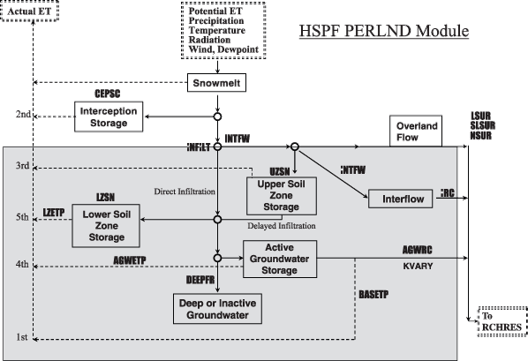
\includegraphics[width=7.33in]{images/hspf_perlnd} \caption{HSPF PERLND Conceptual Model}\label{fig:hspfFig}
\end{figure}

\hypertarget{hydrologic-response-units}{%
\subsection{Hydrologic Response Units}\label{hydrologic-response-units}}

Modeling was performed on discretized landscape units based on common soils, land cover, and slope charcateristics known as hydrologic response units (HRUs). The HRU approach provides a computationally efficient method of pre-computing hydrolgic response for later use. Results for a particular watershed can be calculated by on summing or averaging the results for individual HRUs.

Each combination of parameters were modeled in separate batched simulations. HRUs were designated by a three-digit number according to the following convention:

\begin{itemize}
\tightlist
\item
  First digit: Hydrologic Soil Group Number (0 = A/B, 1 = C, 2 = Saturated)
\item
  Second digit: Land cover (0=Forest, 1=Pasture, 2=Lawn, 5=Impervious),
\item
  Third Digit: Slope (0=Flat, 1=Mod, 2=Steep)
\end{itemize}

For example, a site with Type C soils, with forested land cover, on a moderate slope would be represented by \texttt{101}. This schema allowed for HRUs to be stored as an eight-bit unsigned integer on a Puget-Sound wide raster, minimizing storage size.

\hypertarget{regional-calibrated-parameters}{%
\subsection{Regional Calibrated Parameters}\label{regional-calibrated-parameters}}

Regional calibration factors for the Puget Lowlands Ecoregion were developed the USGS in the 1990s (Dinicola \protect\hyperlink{ref-Dinicola1990}{1990}) and updated by Clear Creek Solutions for use within WWHM (Department of Ecology \protect\hyperlink{ref-DepartmentofEcology2014}{2014}). These parameters, referred to as the `default parameters' by Ecology were used in this study and applied to individual HRUs.

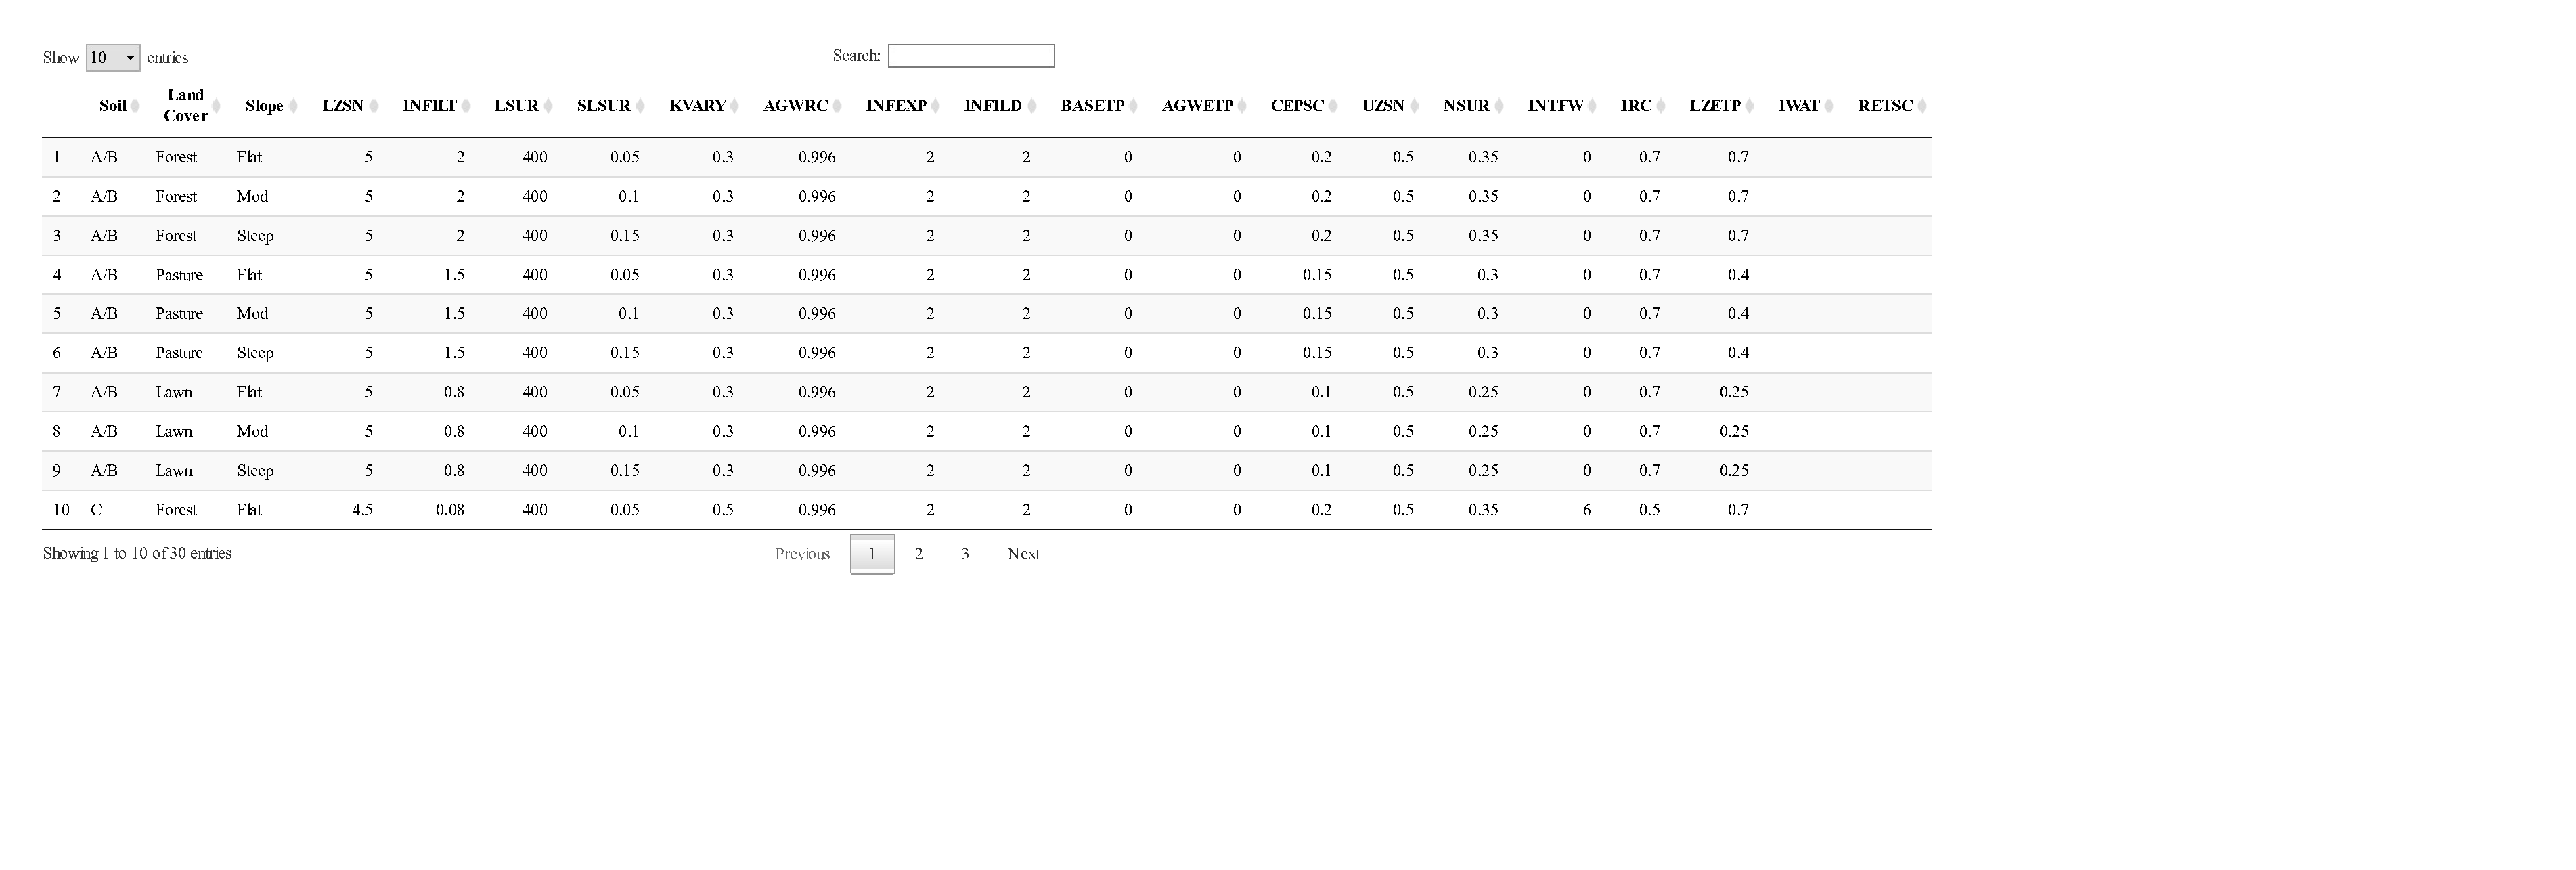
\includegraphics{StormwaterHeatmapTechReference_files/figure-latex/unnamed-chunk-2-1.pdf}

\hypertarget{python-implementation}{%
\subsection{Python Implementation}\label{python-implementation}}

To allow for parallel computations, we used a Python adaption of HSPF developed by David Lambert with funding from the United States Department of Energy, Energy Efficiency \& Renewable Energy, Bioenergy Technologies Office (Lampert \protect\hyperlink{ref-Lampert2019}{2019}). PyHSPF is able to generated HSPF input files, run simulations, and provide HSPF compatible output. Similar to WWHM, we provided separate output files for three flow-paths. Surface flow, interflow, and groundwater flow. In HSPF, these output classes are referred to as \texttt{SURO}, \texttt{INFW}, and \texttt{AGWO} respectively. We developed and ran individual HSPY models for each combination of HRU and Precipitation grid and generated output for each flow patch component. This resulted in 27,990 individual output files.

\hypertarget{data-sources}{%
\section{Data Sources}\label{data-sources}}

\hypertarget{precipitation}{%
\subsection{Precipitation}\label{precipitation}}

A region-wide, simulated precipitation dataset was provided by the University of Washington Climate Impacts Group. Methodology used to develop this dataset is documented in (Mauger et al. \protect\hyperlink{ref-Jr2018}{2018}).The dataset contains modeled hourly precipitation using the GFDL CM3 global climate model and the Representative Concentration Pathways (RCP) 8.5 scenario.

GCM selection based on stormwater applications. Emphasized winter storm drivers.
Downscaled from GFDL CM3. RCP 8.5 (High emissions) ``High-High''
Hourly precipitation developed through application of regional weather model, the Weather Research and Forecasting (WRF, Skamarock et al.~2005).

The GFDL model was chosen by CIG to due to its ability to accurately model winter storm drivers, important for stormwater applications. Combined with the higher emissions scenario, this modeling scenario represents the upper end of expected future climate changes effects.

CIG downscaled GCM results using a statistical-dynamical approach to capture the anticipated changes in extreme events as well as the different drivers of rainfall that affect the Puget Sound Region. Regional simulations were performed using the Weather Research and Forecasting community mesoscale model. This resulted in hourly rainfall predictions at an approximately 12 km grid size across Puget Sound. Predictions were bias-corrected on a quantile-mapping basis (individual mean bias corrections for precipitation in each quantile range) using the historic (1970-2005) WRF data. The WRF Grid in our study area is shown in Figure \ref{fig:wrfGrid}.

\begin{figure}[H]
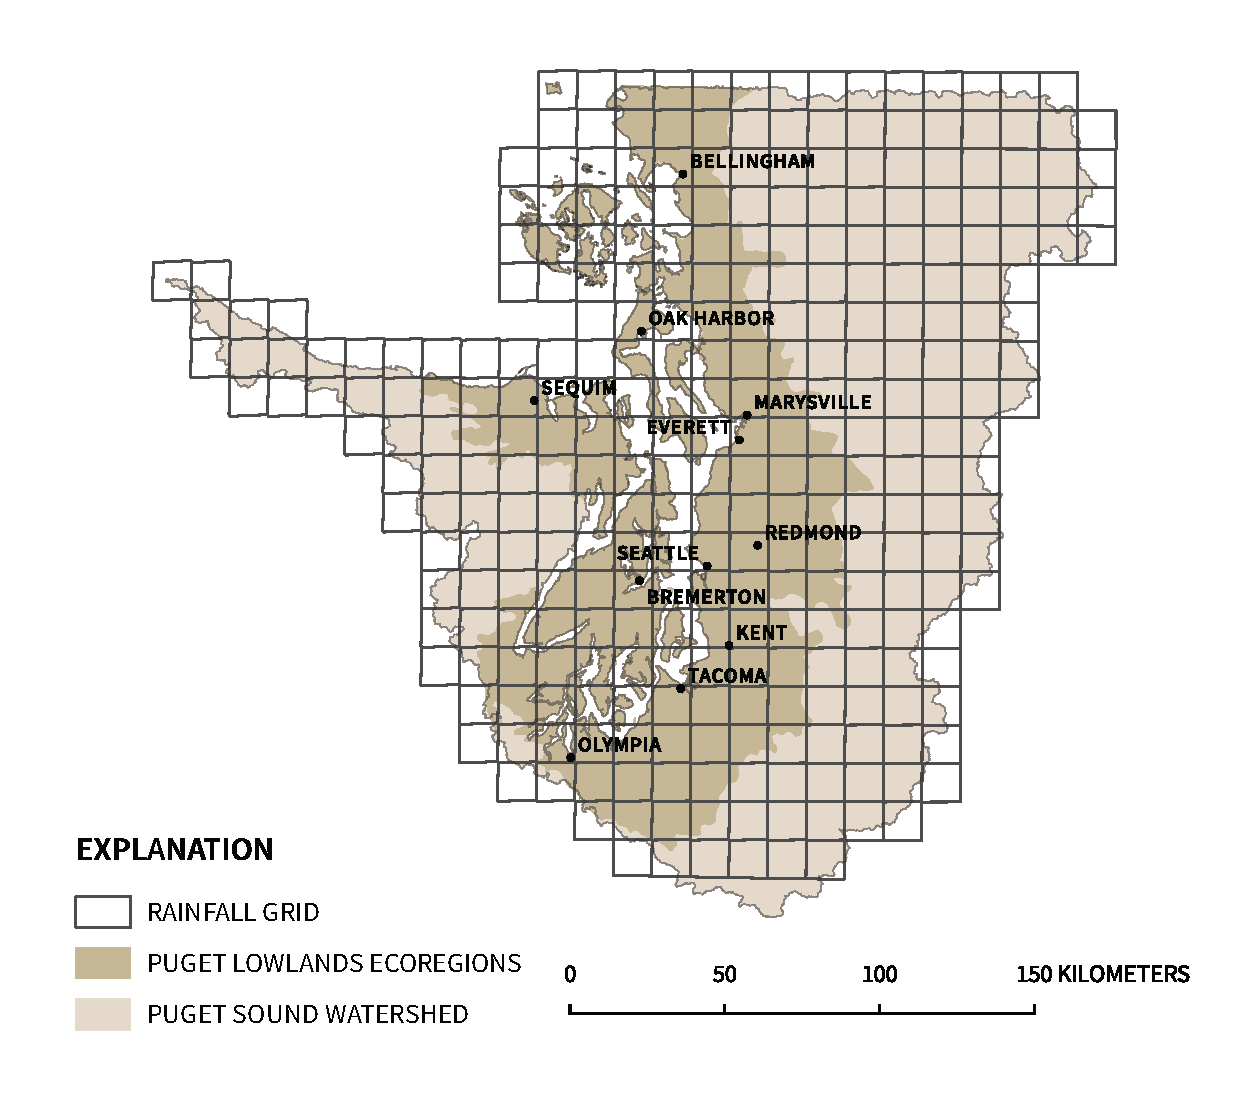
\includegraphics[width=17.28in]{qgis/for_figure} \caption{WRF Forecasting Grid}\label{fig:wrfGrid}
\end{figure}

\hypertarget{potential-evaporation}{%
\subsection{Potential Evaporation}\label{potential-evaporation}}

Gridded potential evaporation estimates were acquired from the forcing data for the North American Land Data Assimilation System (NLDAS2) (NASA Goddard Earth Sciences Data and Information Services Center (GES DISC) \protect\hyperlink{ref-NASAGoddardEarthSciencesDataandInformationServicesCenterGESDISC2019}{2019}). This dataset combines multiple sources of observations to produce estimates of surface climate variables. Evaporation data was derived from the NCEP North American Regional Reanalysis, consisting of a retrospective dataset beginning January 1979 through December 2005. Data were acquired in in 1/8th-degree grid spacing; at an hourly temporal resolution. Average monthly potential evaporation rates were calculated and resampled for each grid cell in the heatmap model domain.

\hypertarget{land-cover}{%
\subsubsection{Land Cover}\label{land-cover}}

Land cover was derived from the Nature Conservancy's high-resolution land cover data set. See Section xx for more informaiton.

\hypertarget{soils}{%
\subsubsection{Soils}\label{soils}}

\hypertarget{gridded-ssurgo-data}{%
\paragraph{Gridded SSURGO Data}\label{gridded-ssurgo-data}}

The primary source of soils data was the Gridded Soil Survey Geographic Database (gSSURGO), (Soil Survey Staff \protect\hyperlink{ref-SoilSurveyStaff2018}{2018}). The gridded soils database contains 10-meter rasterized coverage of surface soils derived from National Cooperate Soil Survey (NCSS) maps. These maps are generally drawn at 1:24000 scale. NCSS designates soils by a ``map-unit name,'' which can be joined with other attribute data. Map units in the study area were joined with the soils component table, containing hydrologic-soil group designations. NCSS classifies hydrologic soil groups according to estimates of runoff potential. Soils are assigned to four groups (A, B, C, and D) and three dual classes (A/D, B/D, and C/D) as defined below:

\begin{itemize}
\item
  \textbf{Group A.} Soils having a high infiltration rate (low runoff potential) when thoroughly wet.
  These consist mainly of deep, well drained to excessively drained sands or gravelly sands.
  These soils have a high rate of water transmission.
\item
  \textbf{Group B.} Soils having a moderate infiltration rate when thoroughly wet. These consist
  chiefly of moderately deep or deep, moderately well drained or well drained soils that have
  moderately fine texture to moderately coarse texture. These soils have a moderate rate of
  water transmission.
\item
  \textbf{Group C.} Soils having a slow infiltration rate when thoroughly wet. These consist chiefly of
  soils having a layer that impedes the downward movement of water or soils of moderately
  fine texture or fine texture. These soils have a slow rate of water transmission.
\item
  \textbf{Group D.} Soils having a very slow infiltration rate (high runoff potential) when thoroughly
  wet. These consist chiefly of clays that have a high shrink-swell potential, soils that have a
  high water table, soils that have a claypan or clay layer at or near the surface, and soils that
  are shallow over nearly impervious material. These soils have a very slow rate of water
  transmission.
\end{itemize}

If a soil is assigned to a dual hydrologic group (A/D, B/D, or C/D), the first letter is for
drained areas and the second is for undrained areas. Only the soils that in their natural
condition are in group D are assigned to dual classes. In certain locations, data were augmented with the SSURGO Value added tables (Soil Survey Staff \protect\hyperlink{ref-SoilSurveyStaff2016}{2016}) using the Potential wetland soil landscapes field.

\hypertarget{oak-ridge-national-laboratory-hysogs250m}{%
\paragraph{Oak Ridge National Laboratory HYSOGs250m}\label{oak-ridge-national-laboratory-hysogs250m}}

In areas where gSSURGO data were not available, we used the Global Hydrologic Soil Groups (HYSOGs250m) for Curve Number-Based Runoff Modeling developed by Oak Ridge National Laboratory {[}RossC.W.L.PrihodkoJ.Y.AnchangS.S.KumarW.Ji2018{]}. This dataset contains world-wide hydrologic soils groups derived at a 250 meter resolution from machine learning predictions. Hydrologic soil groups were given the same designation as the SSURGO data above.

\hypertarget{gaplandfire-data}{%
\paragraph{GAP/LANDFIRE DATA}\label{gaplandfire-data}}

To account for wetlands and saturated soils not included in the above datasets, we used the USGS GAP/LANDFIRE National Terrestrial Ecosystems data set, which includes nationwide vegetation and land cover data.

\hypertarget{slope}{%
\subsubsection{Slope}\label{slope}}

Slope values were calculated from the USGS National Elevation Dataset. Elevations were provided in 1/3 arc-second resolution (approximately 10-meters). Slope was calculated and classified into the following categories, consistent with Ecology guidance:\\
- Flat: \textless{} 5\%\\
- Moderate: 5-15\%\\
- Steep: \textgreater{} 15\%

\hypertarget{verficiation-of-results}{%
\section{Verficiation of Results}\label{verficiation-of-results}}

Results were verified by comparing modeling results to measured stream flow for a gaged watershed in King County. King County operates a stream gage on Madsen Creek, near Renton. The watershed above the gage site is approximately 2,000 acres, with about 25\% imperviousness.

Daily streamflow data for the Madsen Creek watershed was provided by King County for the period 1991-2010. We delineated the watershed above the gaging site using the USGS NHDPLus flow-conditioned raster ({\textbf{???}}).
Using this watershed boundary, we extracted HRUs and associated areas from the stormwater heatmap HRU layer on Google Earth Engine. HRU results and areas are shown in Table \ref{tab:madsenTable}.

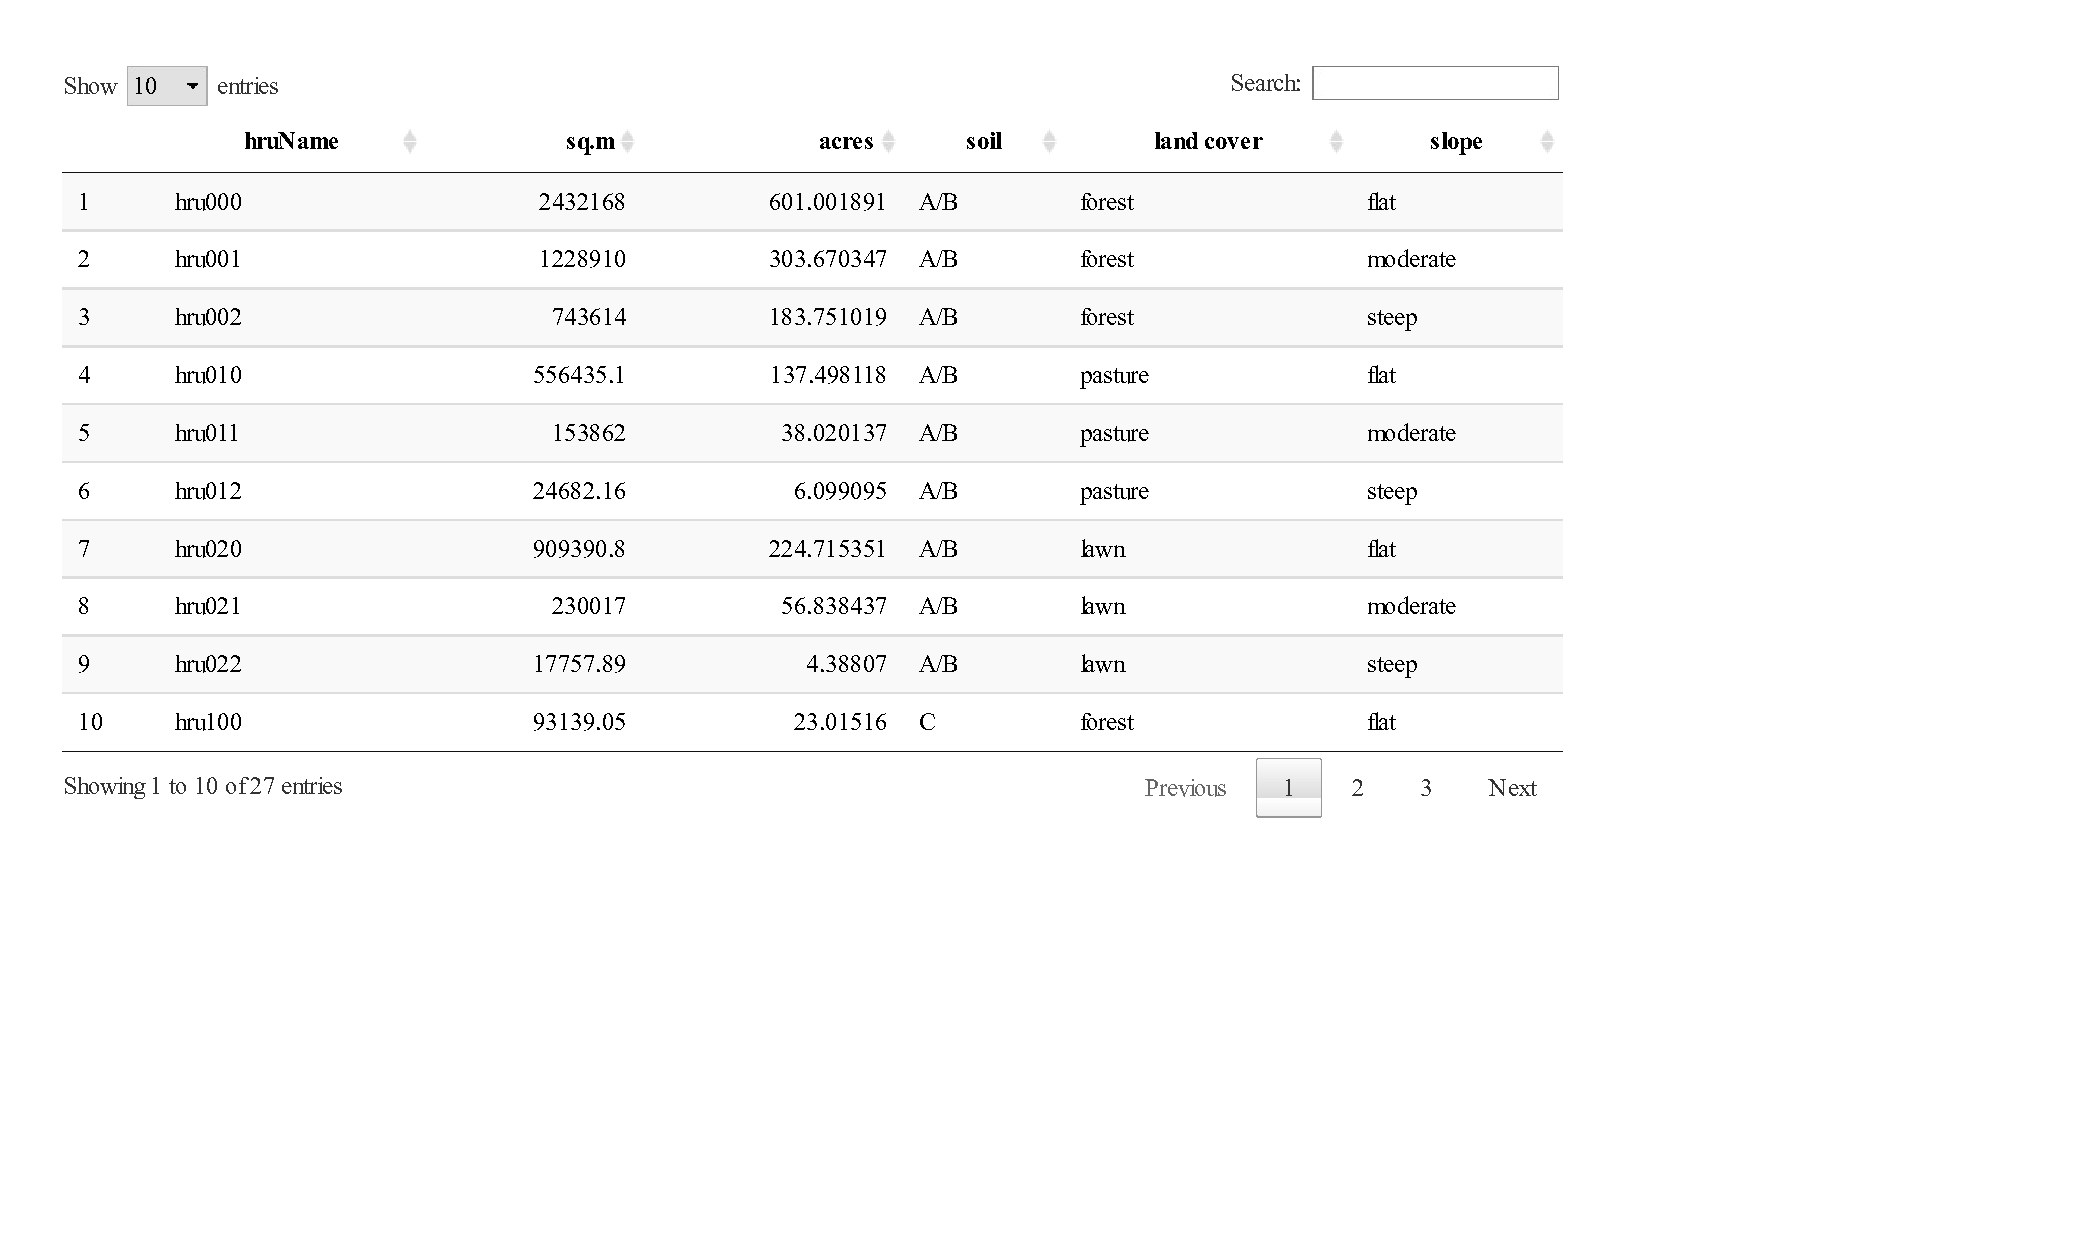
\includegraphics{StormwaterHeatmapTechReference_files/figure-latex/madsenTable-1.pdf}

Modeling results were then queried and aggregated from the BigQuery dataset as described in {[}Tabulated Results via BigQuery{]}. The same HRU values were also run in WWHM for comparison. Both the WWHM and BigQuery results were truncated to have the same period of record as the streamflow data. Only the surface runoff and interflow components were used in this analysis.

Figure @madsenFig shows a comparison of the observed and simulation flow-durations for the Madsen Creek watershed.

\begin{figure}
\centering
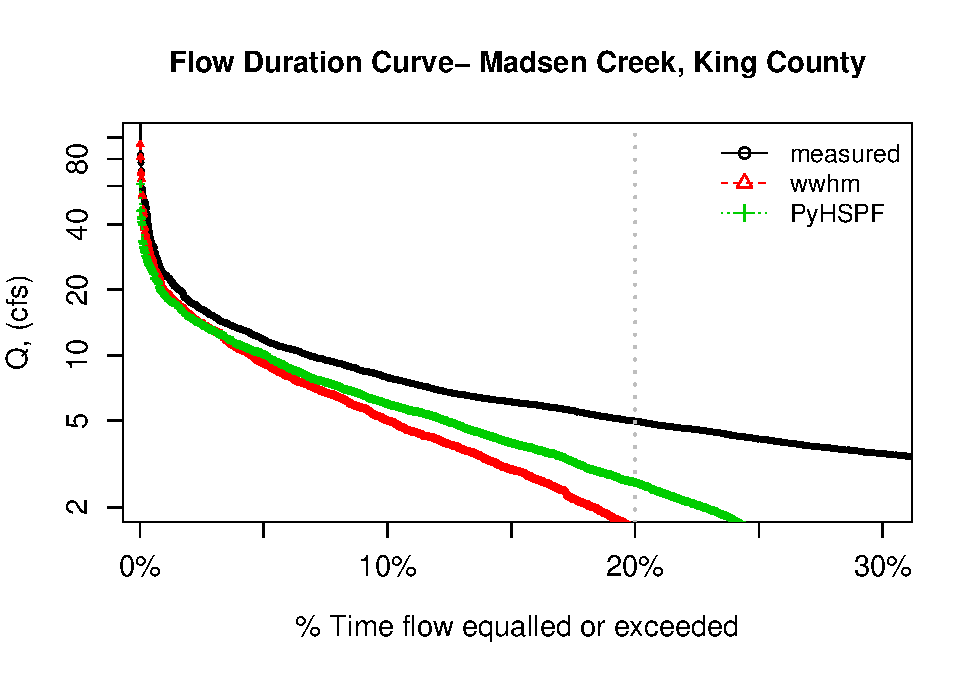
\includegraphics{StormwaterHeatmapTechReference_files/figure-latex/madsenFig-1.pdf}
\caption{\label{fig:madsenFig}Observed and simulated flow-duration curves for Madsen Creek, King County, WA}
\end{figure}

Both the WWHM and HSPY results underpredict actual streamflow primarly because baseflow was not simulated. This is expected, since both models exclude groundwater contributions. However, the results show good agreement between both simulated datasets over the full duration of simulations. Note that the simulations use different precipitation and potential evaporation datasets and are not expected to match.

\hypertarget{spatially-aggregated-results}{%
\section{Spatially Aggregated Results}\label{spatially-aggregated-results}}

Since the HSPY model is a lumped parameter model, results can be calculated for HRU/precipitation grids individually and then aggregated after calculation.

The stormwater heatmap contains two spatial aggregates of hydrology results: Mean Annual Runoff for the historic period (1970-1999) and a new index, termed the Flow Duration Index.

\hypertarget{mean-annual-runoff-1970-1999}{%
\subsection{Mean Annual Runoff (1970-1999)}\label{mean-annual-runoff-1970-1999}}

Mean annual runoff for each HRU/grid combination was aggregated from BigQuery for the historic period of record (1970-1999). Consistent with Ecology guidance for stormwater projects, only the surface flow components, \texttt{SURO} and \texttt{IFWO} were used. \texttt{AGWO}, deep groundwater flow, was not included in this calculation.

Total runoff was calculated for each year/hru/grid combination in the period of record, then averaged by hru/grid combination.

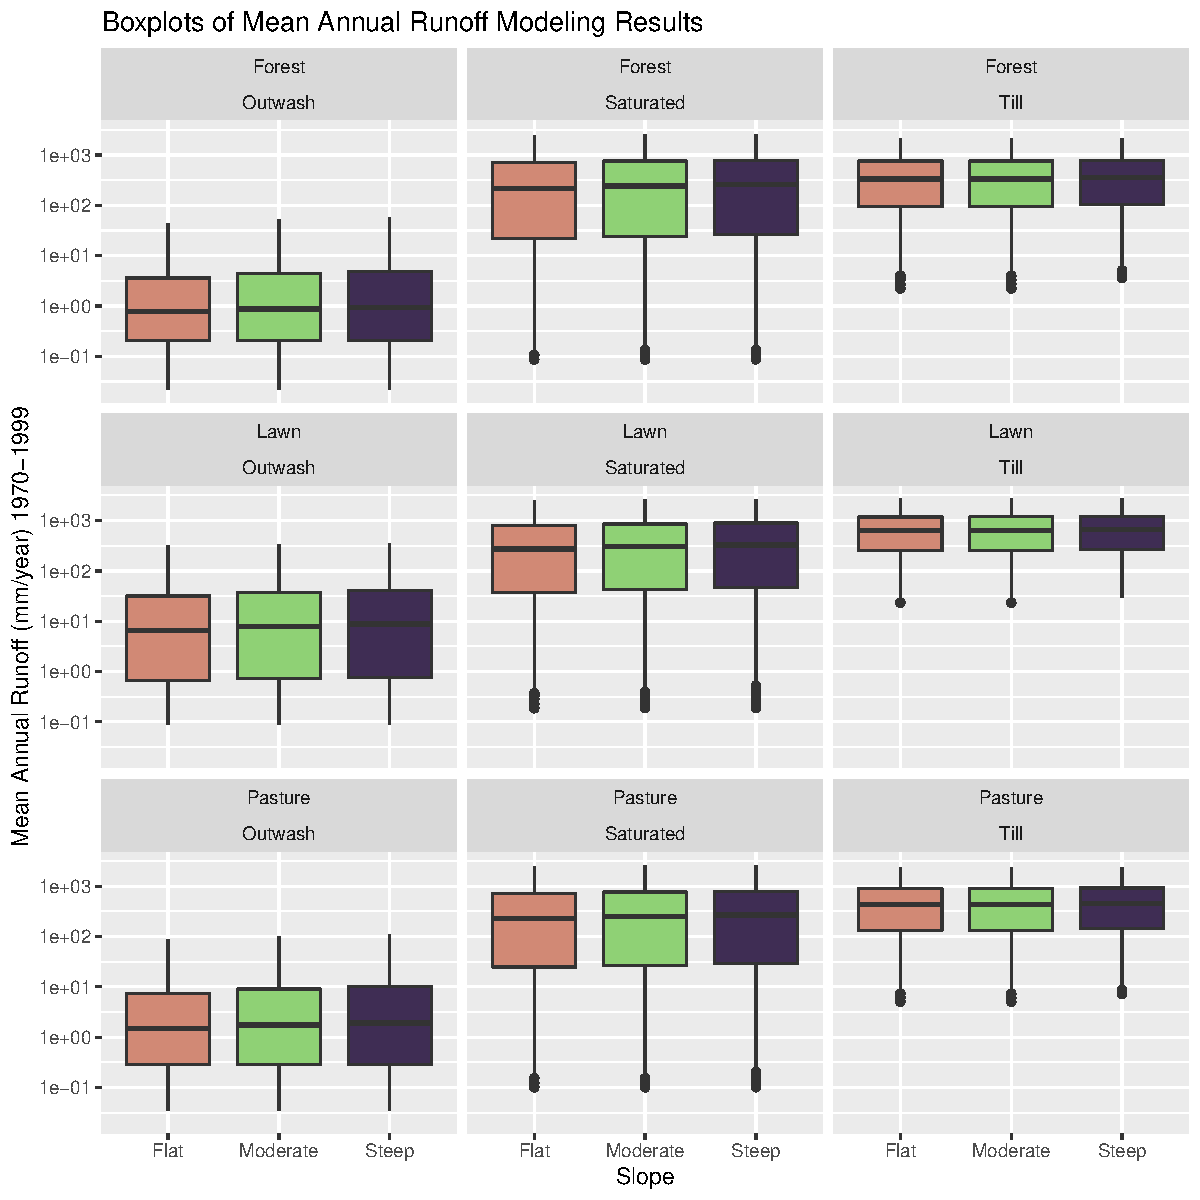
\includegraphics{StormwaterHeatmapTechReference_files/figure-latex/unnamed-chunk-4-1.pdf}

\hypertarget{flow-duration-index}{%
\subsection{Flow Duration Index}\label{flow-duration-index}}

\hypertarget{ecology-performance-standards}{%
\subsubsection{Ecology Performance Standards}\label{ecology-performance-standards}}

Ecology Stormwater Guidance includes flow-related performance standards to protect receiving waters from degradation caused by changes in the hydrologic regime due to development. These performance standards rely on flow-duration matching, whereby flow durations from developed land are required to match pre-developed flow-durations for a range of discharge values.The flow duration standard is intended to prevent flashy flows in receiving stream channels.

\hypertarget{calculation-of-the-index}{%
\subsubsection{Calculation of the Index}\label{calculation-of-the-index}}

We developed an index representing the magnitude of change to the flow-duration curve between flow thresholds.Thresholds were chosen based on Ecology's LID and Flow Control Standards (Department of Ecology \protect\hyperlink{ref-DepartmentofEcology2014}{2014}), which require flow-duration matching over the range between 8 percent of the 2-year peak discharge (lower threshold of the LID standard) up to the 50-year peak discharge (upper threshold of the flow-control standard).

The flow discharge index is calculated by summing the discharge over the simulation period between a high-flow and low-flow threshold. Figure \ref{fig:fdrfig} illustrates the summation of flow-duration values used in calculating this index.

\begin{figure}
\centering
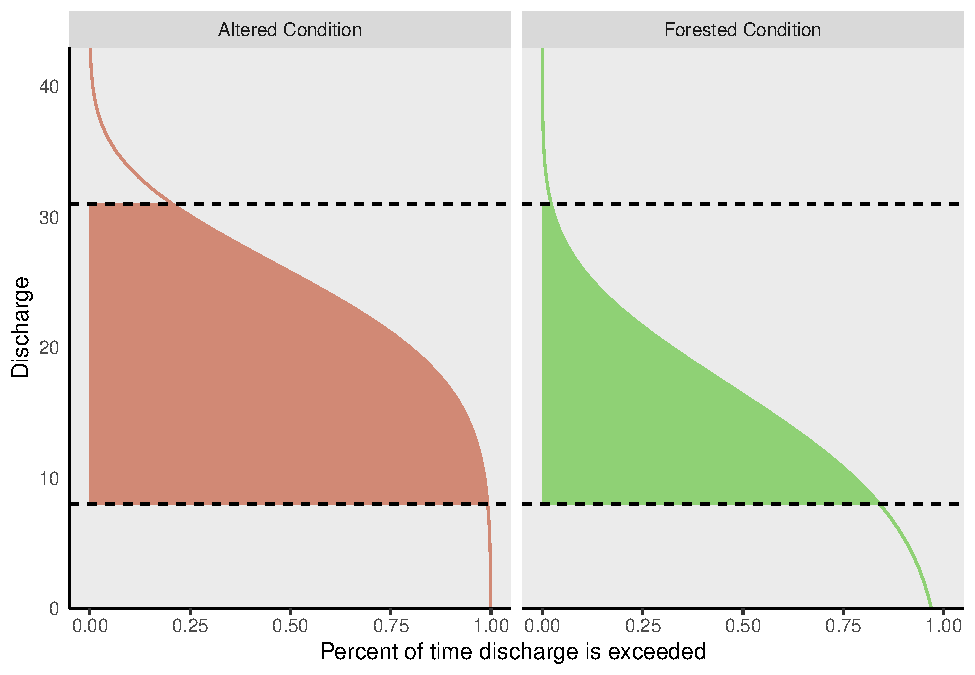
\includegraphics{StormwaterHeatmapTechReference_files/figure-latex/fdrfig-1.pdf}
\caption{\label{fig:fdrfig}Example flow duration curves of altered and forested land covers}
\end{figure}

The flow duration index can be described by Equation \eqref{eq:fdr}.

\begin{equation}
  \ln\left(\frac{\sum_{ }^{ }q_{current}\Delta t}{\sum_{ }^{ }q_{forest}\Delta t}+1\right)
  \label{eq:fdr}
\end{equation}0.08Q\_2\textless q~\le~Q\_\{50\};0.08Q\_2\textless q~\le~Q\_\{50\}

Where q\textsubscript{current} is the simulated discharge for current or altered conditions and q\textsubscript{forest} is the predevelopment or forested conditions. One is added to this ratio and the logarithm is taken to produce an index that generally falls between 1 and 10. This index is then applied to hru/grid combinations in the stormwater heatmap to produce a spatially explicit mapping of flow alteration.

\hypertarget{flow-duration-summary-index}{%
\subsubsection{Flow Duration Summary Index}\label{flow-duration-summary-index}}

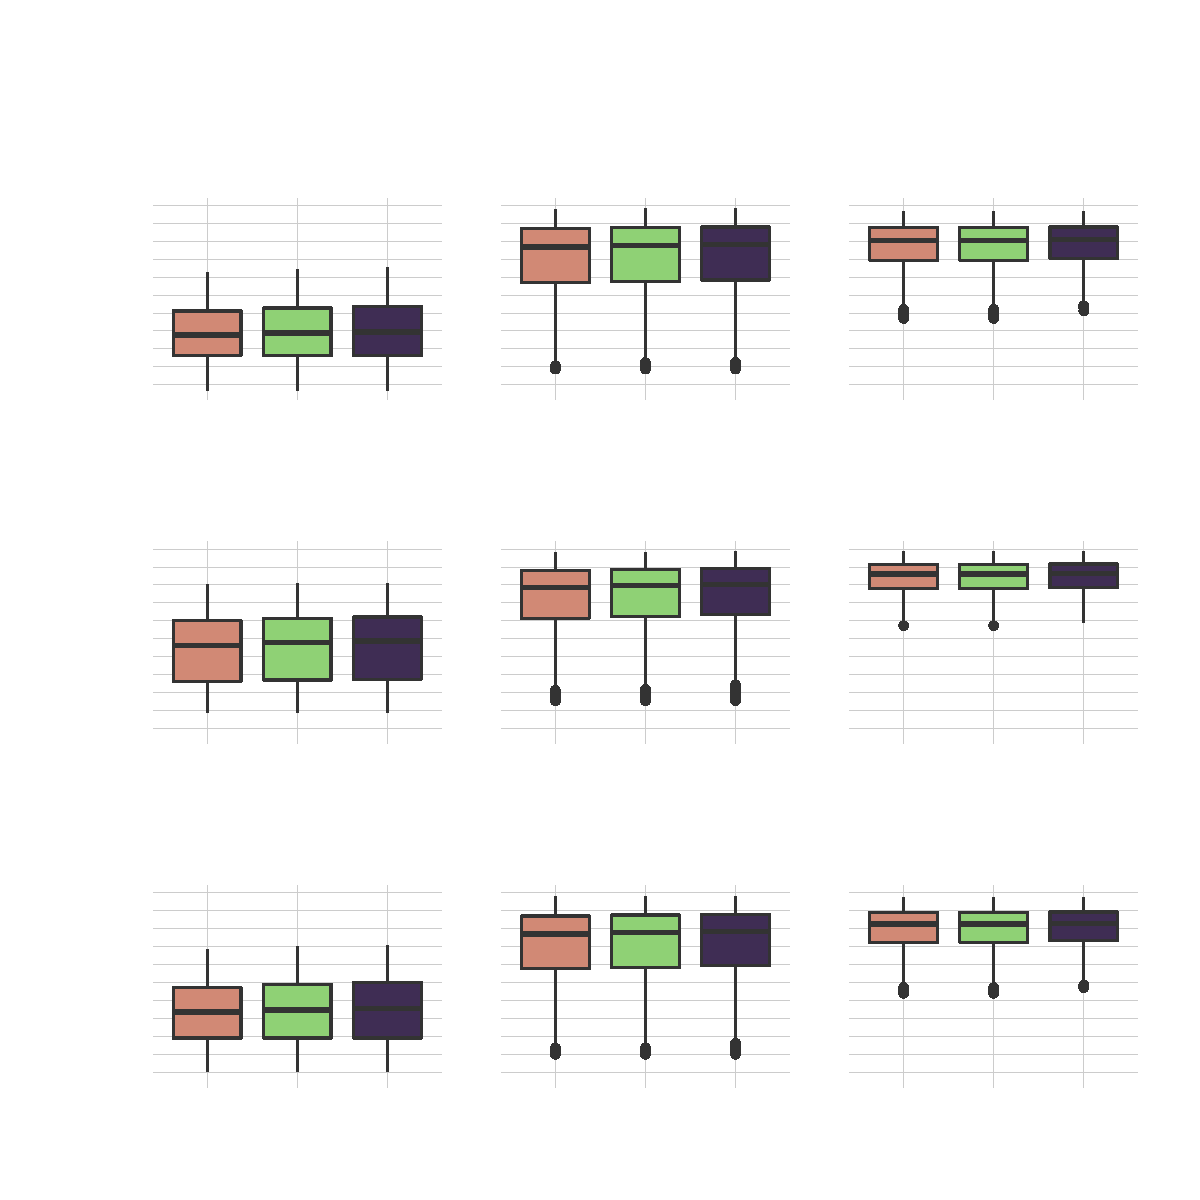
\includegraphics{StormwaterHeatmapTechReference_files/figure-latex/unnamed-chunk-5-1.pdf}
\#\# Tabulated Results via BigQuery

Tabulated hydrology results are available via \href{https://cloud.google.com/bigquery}{Google BigQuery}, a cloud-based relational database that includes a distributed SQL engine. The data are located on the \href{https://console.cloud.google.com/bigquery?project=tnc-data-v1}{\texttt{tnc-data-v1} data bucket} (sign-in require). The table is named \texttt{tnc-data-v1:hydrology.gfdl.} BigQuery supports several client libraries. See \url{https://cloud.google.com/bigquery/docs/reference/libraries} for a list of supported clients libraries.

Using R, the tnc-data-v1 databucket can be accessed through a database connection using the DBI package:

\hypertarget{schema}{%
\subsection{Schema}\label{schema}}

The table schema are shown in Table \ref{tab:schemaTable}.

\begin{table}

\caption{\label{tab:schemaTable}BigQuery Table Schema for `tnc-data-v1:hydrology.gfdl.`}
\centering
\begin{tabular}[t]{l|l|l}
\hline
Fieldname & Type & Description\\
\hline
grid & STRING & WRF Grid ID Number\\
\hline
year & INTEGER & Year of Simulation\\
\hline
month & INTEGER & Month of Simulation\\
\hline
comp & STRING & HSPF Runoff component (AGWO, IFWO, SURO)\\
\hline
hru000 … hru252 & STRING & Runoff (mm) (one column for each HRU)\\
\hline
Datetime & TIMESTAMP & Simulation Hour (UTC)\\
\hline
simulation\_day & INTEGER & Day of simulation (01-Jan-1970 = Day 1)\\
\hline
simulation\_day & INTEGER & Day of simulation (01-Jan-1970 = Day 1)|\\
\hline
\end{tabular}
\end{table}

\hypertarget{querying-tabulated-results}{%
\subsection{Querying Tabulated Results}\label{querying-tabulated-results}}

The data may be queried through Google Cloud Platform directly, or through a number of available software libraries. Queries are performed through standard SQL language. Some example queries are provided below.

Get all surface flow components from the SeaTac precipitation grid (ID16\_V7) for the years 1970-1999:

Get the annual peak flow for surface flow components from the SeaTac precipitation grid (ID16\_V7) for the years 1970-1999:

\hypertarget{querying-geometry}{%
\subsection{Querying Geometry}\label{querying-geometry}}

Google BigQuery supports PostGIS geometry functions (see \url{https://cloud.google.com/bigquery/docs/reference/standard-sql/geography_functions} for instructions).

Grid geometries are available from the \texttt{tnc-data-v1.gfdl.geometry} table on Big Query. The table schema is as follows:

\begin{longtable}[]{@{}lllll@{}}
\toprule
Fieldname & Type & Description & &\tabularnewline
\midrule
\endhead
grid & STRING & WRF Grid ID Number & &\tabularnewline
xy & GEOGRAPHY & Centroid of the grid (PostGIS point) ) & &\tabularnewline
geohash & String & PostGIS geohash string approximating grid boundary & &\tabularnewline
geometry & STRING & Well known text format of the grid boundary & &\tabularnewline
\bottomrule
\end{longtable}

An example query to return the Grid ID covering the Seattle Center:

Returns the grid ID pertaining to this location:

\begin{verbatim}
Row  grid
-----------
 1  ID16_V9
\end{verbatim}

\hypertarget{water-quality-statistics}{%
\chapter{Water Quality Statistics}\label{water-quality-statistics}}

\hypertarget{references}{%
\chapter{References}\label{references}}

\hypertarget{refs}{}
\leavevmode\hypertarget{ref-Anan2002}{}%
Anan, Y; Kunito T, T Ikemoto, R Kubota, I Watanabe, S Tanabe, N Miyazaki, and E Petrov. 2002. ``Elevated concentrations of trace elements in Caspian seals (Phoca caspia) found stranded during the mass mortality event in 2000.'' \emph{Environmental Contamination \& Toxicology} 42: 354--62.

\leavevmode\hypertarget{ref-Anderson2007}{}%
Anderson, B, J Hunt, B Phillips, B Thompson, S Lowe, i K Tabersk, and R Carr. 2007. ``Patterns and trends in sediment toxicity in the San Francisco Estuary.'' \emph{Environmental Research} 105: 145--55.

\leavevmode\hypertarget{ref-Arkoosh2001}{}%
Arkoosh, M, E Clemons, P Huffman, A Kagley, E Casillas, N Adams, H Sanborn, T Collier, and J Stein. 2001. ``Increased Susceptibility of Juvenile Chinook Salmon to Vibriosis after Exposure to Chlorinated and Aromatic Compounds Found in Contaminated Urban Estuaries.'' \emph{Journal of Aquatic Animal Health} 13 (3): 257--68.

\leavevmode\hypertarget{ref-Baldwin2011}{}%
Baldwin, D, C Tatara, and N Scholz. 2011. ``Copper induced olfactory toxicity in salmon and steelhead: Extrapolation across species and rearing environments.'' \emph{Aquatic Toxicology.} 101 (1): 295--97.

\leavevmode\hypertarget{ref-County2014}{}%
County, King. 2014. ``Development of a Stormwater Retrofit Plan for Water Resources Inventory Area (WRIA) 9: Comprehensive Needs and Cost Assessment and Extrapolation to Puget Sound.'' Prepared by Simmonds J; Wright O, King County Department of Natural Resource; Parks, Water; Land Resources Division.

\leavevmode\hypertarget{ref-DepartmentofEcology2014}{}%
Department of Ecology. 2014. ``Stormwater Management Manual for Western Washington,'' 1192.

\leavevmode\hypertarget{ref-Dinicola1990}{}%
Dinicola, Richard S. 1990. ``Characterization and simulation of rainfall-runoff relations for headwater basins in western King and Snohomish Counties, Washington.'' \emph{Water-Resources Investigations Report} 89-4052: 52 p. \url{https://pubs.er.usgs.gov/publication/wri894052}.

\leavevmode\hypertarget{ref-Feist2017}{}%
Feist, Blake E., Eric R. Buhle, David H. Baldwin, Julann A. Spromberg, Steven E. Damm, Jay W. Davis, and Nathaniel L. Scholz. 2017. ``Roads to ruin: Conservation threats to a sentinel species across an urban gradient.'' \emph{Ecological Applications} 27 (8): 2382--96. \url{https://doi.org/10.1002/eap.1615}.

\leavevmode\hypertarget{ref-Gaw2014}{}%
Gaw, S, K Thomas, and T Hutchinson. 2014. ``Sources, impacts and trends of pharmaceuticals in the marine and coastal environment.'' \emph{Philosophical Transactions of the Royal Society B: Biological Sciences} 369: 20130572.

\leavevmode\hypertarget{ref-Incardona2011}{}%
Incardona, J, T Linbo, and N Scholz. 2011. ``Cardiac toxicity of 5-ring polycyclic aromatic hydrocarbons is differentially dependent on the aryl hydrocarbon receptor 2 isoform during zebrafish development.'' \emph{Toxicology and Applied Pharmacology} 257 (2): 242--49.

\leavevmode\hypertarget{ref-Jarvis2015}{}%
Jarvis, T., and G. Bielmyer-Fraser. 2015. ``Accumulation and effects of metal mixtures in two seaweed species.'' \emph{Comparative Biochemistry and Physiology, Part C. Toxicology and Pharmacology} 171: 28--33.

\leavevmode\hypertarget{ref-Kayhanian2012}{}%
Kayhanian, M, B Fructman, J Gulliver, C Montanaro, E Ranieri, and S Wuertz. 2012. ``Review of highway runoff characteristics: Comparative analysis and universal implications.'' Water Research. Vol. 46, pp.'' \emph{Water Research}, 6609--24.

\leavevmode\hypertarget{ref-Lampert2019}{}%
Lampert, David. 2019. ``PyHSPF.'' \url{https://github.com/djlampert/PyHSPF}.

\leavevmode\hypertarget{ref-Levin}{}%
Levin, P, E Howe, and J Robertson. n.d. ``Impacts of stormwater on coastal ecosystems: the need to match the scales of management objectives and solutions.'' \emph{Philosophical Transactions of the Royal Society B: Biological Sciences}.

\leavevmode\hypertarget{ref-Lyngby1984}{}%
Lyngby, J, and H Brix. 1984. ``Seasonal and environmental variation in cadmium, copper, lead, and zinc concentrations in eelgrass (Zostera marina L.) in the Limfjord, Denmark.'' \emph{Aquatic Botany} 54: 100--106.

\leavevmode\hypertarget{ref-Jr2018}{}%
Mauger, G. S., J. S. Won, K. Hegewisch, C. Lynch, R. Lorente Plazas, Salathe, and E. P. Salathé Jr. 2018. ``New Projections of Changing Heavy Precipitation in King County.''

\leavevmode\hypertarget{ref-McIntyre2015}{}%
McIntyre, J, J Davis, C Hinman, K Macneale, B Anulacion, N Scholz, and J Stark. 2015. ``Soil bioretention protects juvenile salmon and their prey from the toxic impacts of urban stormwater runoff.'' \emph{Chemosphere} 132: 213--19.

\leavevmode\hypertarget{ref-Meador2006}{}%
Meador, J, F Sommers, and SC Ylitalo. 2006. ``Altered growth and related physiological responses in juvenile Chinook salmon (Oncorhynchus tshawytscha) from dietary exposure to polycyclic aromatic hydrocarbons (PAHs).'' \emph{Canadian Journal of Fisheries and Aquatic Sciences} 63: 2364--76.

\leavevmode\hypertarget{ref-NASAGoddardEarthSciencesDataandInformationServicesCenterGESDISC2019}{}%
NASA Goddard Earth Sciences Data and Information Services Center (GES DISC). 2019. ``NLDAS-2: North American Land Data Assimilation System Forcing Fields.''

\leavevmode\hypertarget{ref-Palmer2019}{}%
Palmer, Margaret, and Albert Ruhi. 2019. ``Linkages between flow regime, biota, and ecosystem processes: Implications for river restoration.'' \emph{Science} 365 (6459): eaaw2087.

\leavevmode\hypertarget{ref-Rice2000}{}%
Rice, C, M Myers, M Willis, B French, and E Casillas. 2000. ``From sediment bioassay to fish biomarker -- connecting the dots using simple trophic relationships.'' \emph{Marine Environmental Research} 50: 527--22.

\leavevmode\hypertarget{ref-Ross2000}{}%
Ross, P, Ellis G, M Ikonomou, L Barrett-Lennard, and R Addison. 2000. ``High PCB concentrations in freeranging Pacific killer whales, Orcinus orca: Effects of age, sex and dietary preference.'' \emph{Marine Pollution Bulletin} 40 (6): 504--15.

\leavevmode\hypertarget{ref-Scholz2011}{}%
Scholz, N, M Myers, S McCarthy, J Labenia, and J McIntyre. 2011. ``Recurrent Die-Offs of Adult Coho Salmon Returning to Spawn in Puget Sound Lowland Urban Streams.'' \emph{PLoS ONE} 6 (12): e28013.

\leavevmode\hypertarget{ref-SoilSurveyStaff2016}{}%
Soil Survey Staff. 2016. ``National Value Added Look Up (valu) Table Database for the Gridded Soil Survey Geographic (gSSURGO) Database for the United States of America and the Territories, Commonwealths, and Island Nations served by the USDA-NRCS.''

\leavevmode\hypertarget{ref-SoilSurveyStaff2018}{}%
---------. 2018. ``Gridded Soil Survey Geographic (gSSURGO) Database for Washington.'' \url{https://gdg.sc.egov.usda.gov/}.

\leavevmode\hypertarget{ref-USEPA2019}{}%
United States Environmental Protection Agency. 2019. ``National rivers and streams assessment 2008-2019: A collaborative survey.'' U.S. Environmental Protection Agency.

\leavevmode\hypertarget{ref-Walsh2005}{}%
Walsh, Christopher J., Allison H. Roy, Jack W. Feminella, Peter D. Cottingham, Peter M. Groffman, and Raymond P. Morgan. 2005. ``The urban stream syndrome: Current knowledge and the search for a cure.'' \emph{Journal of the North American Benthological Society} 24 (3): 706--23. \url{https://doi.org/10.1899/04-028.1}.

\leavevmode\hypertarget{ref-WashingtonStateDepartmentofEcology2011}{}%
Washington State Department of Ecology. 2011. ``Toxics in Surface Runoff to Puget Sound: Phase 3 Data and Load Estimates.'' Prepared by Herrerra Environmental COnsultants, Inc.: Washington Department of Ecology.

\leavevmode\hypertarget{ref-WashingtonStateDepartmentofEcologyandWashingtonDepartmentofHealth2012}{}%
Washington State Department of Ecology and Washington Department of Health. 2012. ``PAH Chemical Action Plan.'' Prepared Davies H, Stone A, Grice J, Patora K, Kadlex M, Delistraty D, Norton D,; White J.: Washington Department of Ecology; Washington Department of Health.

\leavevmode\hypertarget{ref-WDFW2011}{}%
WDFW. 2011. ``Toxic Contaminants in Harbor Seal (Phoca vitulina) Pups from Puget Sound.'' Prepared by Noell M, Ross P, Jeffries S, Lance M: Washington Department of Fish; Wildlife.

\end{document}
